\documentclass[12pt]{article}
\usepackage[usenames]{color} %used for font color
\usepackage{amssymb}
\usepackage{pho-equation}
\usepackage[assignment]{pho-format}

%\usepackage{url} % Formatting packages
\usepackage{hyperref} % Required for adding links and customizing them
\definecolor{linkcolour}{rgb}{0,0.2,0.6} % Link color
\hypersetup{colorlinks,breaklinks,urlcolor=linkcolour,linkcolor=linkcolour} % Set link colors throughout the document


\newcommand{\githubRepoNameFormat}[1]{ \textsl{\footnotesize#1} }
%\github{real-URL}{display-name}
%\newcommand{\github}[2]{\faGithub\href{#1}{#2}}
\newcommand{\github}[2]{\href{#1}{\githubRepoNameFormat{#2}}}

%\githubFromShortName{githubUser}{repoName}{displayName}
\newcommand{\githubFromShortName}[3]{\github{https://github.com/#1/#2}{#3}}

%\phoGithub{repoName}{displayName}
%\newcommand{\phoGithub}[2]{\githubFromShortName{CommanderPho}{#1}{#2 (Private)}}
\newcommand{\phoGithub}[2]{\githubFromShortName{CommanderPho}{#1}{#2}}



\title{NSCI 613 - Lab 3}
\author{\phoName}
\subject{ NSCI 613 - Neurophysiology and Computational Neuroscience }
%\studentID{2437149}


\begin{document}
\maketitle
%\vfill
%All source code for this assignment is available in my Github repository: \phoGithub{NSCI-613-Lab-2}{https://github.com/CommanderPho/NSCI-613-Lab-2}

\updateheaders
\clearpage

%\slntParagraph{ Increasing the delay of the second current pulse from $9[ms]$ up in $0.1[ms]$ increments, we find that a delay of approximately $10.3[ms]$ is the minimum refractory time between action potential events evoked by a current pulse of the same magnitude. See Figure \ref{fig:P1} for the voltage curve.}


%\begin{figure}[H]
%\centering
%\includegraphics[width=0.9\textwidth]{Results/P1}
%\caption{\label{fig:P1} Voltage Plots used to determine the minimum refractory time between action potential events for P1. }
%\end{figure}



% P1
\Question{Neurons in Action - Unmyelinated Axon Tutorial}

%% P1.A
\subQuestion{Velocity as a function of axon diameter}

\begin{figure}[H]
\centering
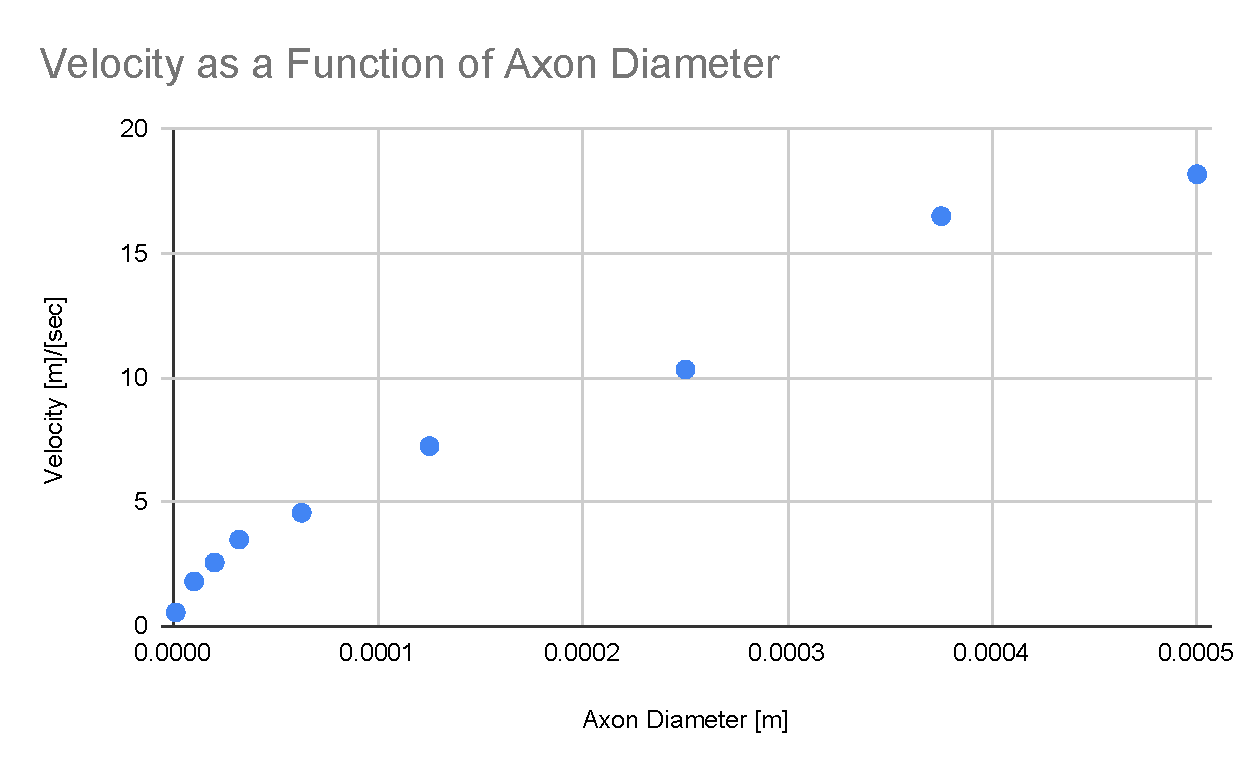
\includegraphics[width=0.9\textwidth]{Results/1a-1}
\caption{\label{fig:P1a1} Plot of axon diameter vs. conductance velocity }
\end{figure}

%\begin{table}[h!]
%\begin{tabular}{|l|l|l|}
%\hline
%Voltage Step [mV] & Peak $I_{\text{Na}} \rfrac{mA}{\text{cm}^2}$ & Peak $g_{\text{Na}}$ \\ \hline\hline
%-5                & -1.5738                                   & 0.023                                    \\ \hline
%+100              & 2.275                                    & 0.051                                      \\ \hline
%\end{tabular}
%\caption{Subthreshold Oscillation Values for  }
%\label{table:3}
%\end{table}


\begin{table}[h!]
\begin{tabular}{|l|l|l|l|l|}
                  & \multicolumn{2}{l}{Zero Time [ms]} &                     &                     \\
Axon Diameter [m] & 0.1              & 0.9             & Time Difference [sec] & Velocity $\rfrac{m}{\text{sec}}$ \\ \hline\hline
0.0005            & 0.71             & 1.15            & 0.00044             & 18.18181818         \\
0.000375          & 0.975            & 1.46            & 0.000485            & 16.49484536         \\
0.00025           & 0.55             & 1.325           & 0.000775            & 10.32258065         \\
0.000125          & 0.975            & 2.08            & 0.001105            & 7.239819005         \\
0.0000625         & 0.525            & 2.28            & 0.001755            & 4.558404558         \\
0.000032          & 1.53             & 3.83            & 0.0023              & 3.47826087          \\
0.00002           & 0.9              & 4.03            & 0.00313             & 2.555910543         \\
0.00001           & 0.975            & 5.43            & 0.004455            & 1.795735129         \\
0.000001          & 1.975            & -               & -                   & -                  
\end{tabular}
\caption{Zero-crossing times measured at two different distances (0.1 and 0.9) from the stimulation location. Velocity was calculated using $v = \frac{0.008}{\Delta t}$ where 0.008 is the displacement distance along the axon between the two curves. }
\label{table:1}
\end{table}


%% P1.B
\subQuestion{Relationship between axon diameter and velocity. } 

\par Transforming the x-axis d using the relation $\defn{z}{\sqrt{d}}$ we can compute the linear line-of-best-fit for the transformed coordinates (as is shown in Figure $\ref{P1a2}$), and then convert back to the original.


\begin{figure}[H]
\centering
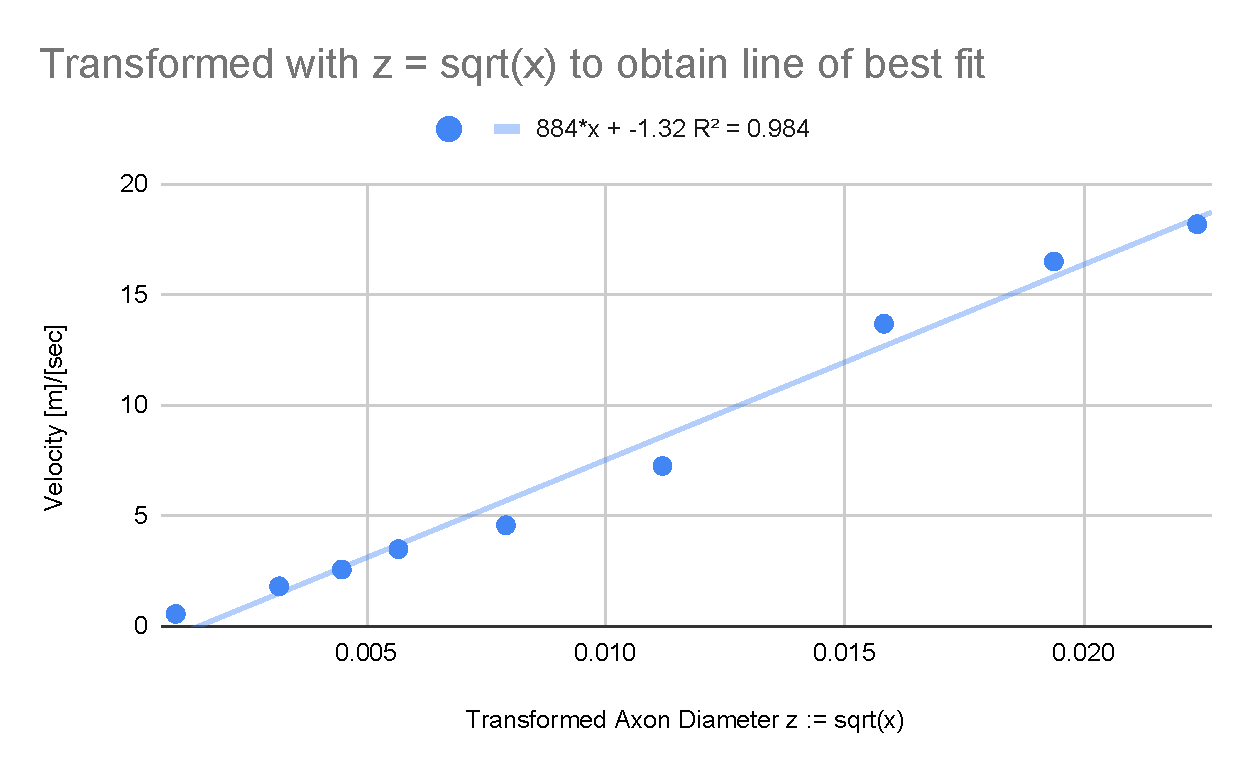
\includegraphics[width=0.9\textwidth]{Results/1a-2}
\caption{\label{fig:P1a2} Plot of transformed axon diameter vs. conductance velocity that was used to get the linear line-of-best-fit which was used to compute K.}
\end{figure}


\work{$y = 870 z + -1.7$}
\work{$y = 870 \sqrt{d} + -1.7$}
\work{From this we can conclude that if $v = K \sqrt{d}$, then}
\sln{K = 870}

\slntParagraph{ We find that curve does follow the predicted relationship and is fit by the form: $v = 870 \sqrt{d} + -1.7$. }


 





% P2
\Question{Neurons in Action - Myelinated Axon Tutorial}

%% P2.A
\subQuestion{Degree of Myelination and Conductance Velocity} 

\begin{figure}[H]
\centering
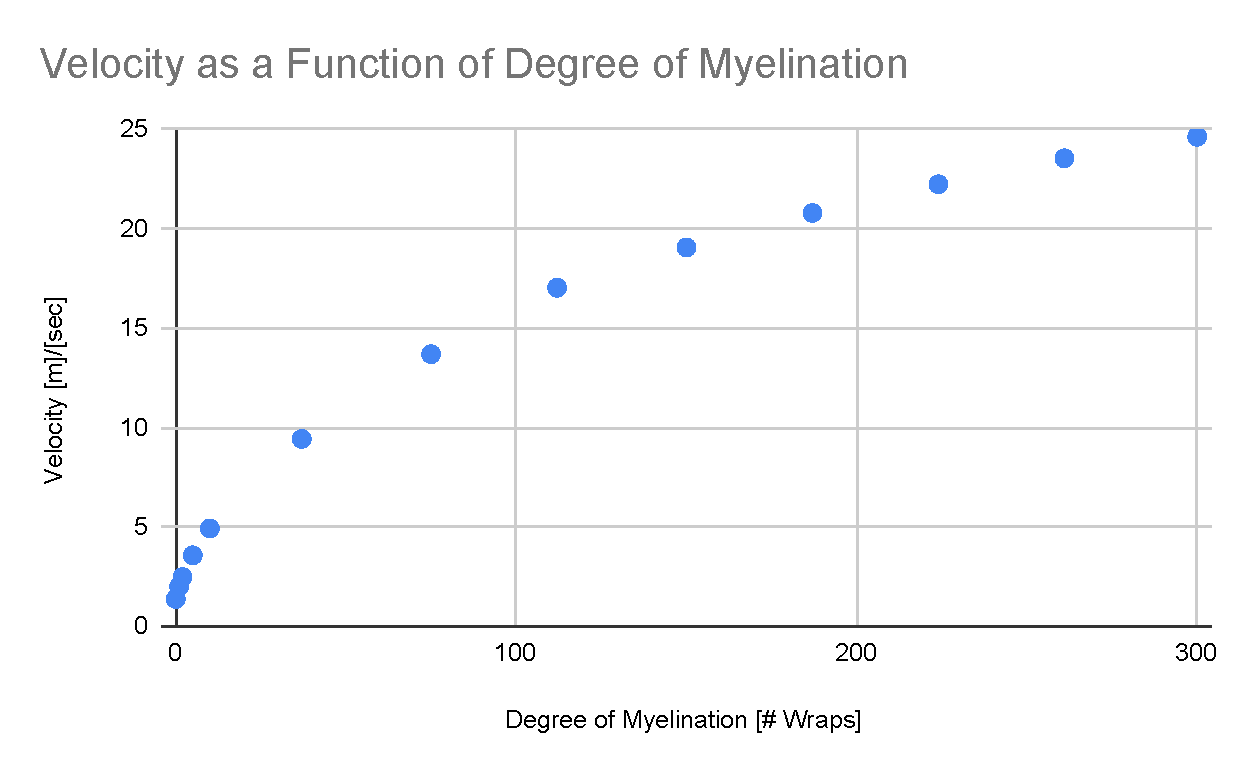
\includegraphics[width=0.9\textwidth]{Results/2a}
\caption{\label{fig:P2} Plot of the degree of myelination (as characterized by the number of wraps) vs. the conductance velocity.}
\end{figure}

\begin{table}[h!]
\begin{tabular}{|l|l|l|l|l|}
                  & \multicolumn{2}{l}{Zero Time [ms]} &                     &                     \\
Degree of Myelination [\# Wraps] & 0.1              & 0.9             & Time Difference [sec] & Velocity $\rfrac{m}{\text{sec}}$ \\ \hline\hline
37                          & 0.16  & 1.01  & 0.00085               & 9.411764706        \\
75                          & 0.29  & 0.875 & 0.000585              & 13.67521368        \\
112                         & 0.27  & 0.74  & 0.00047               & 17.0212766         \\
150                         & 0.25  & 0.67  & 0.00042               & 19.04761905        \\
187                         & 0.24  & 0.625 & 0.000385              & 20.77922078        \\
224                         & 0.23  & 0.59  & 0.00036               & 22.22222222        \\
261                         & 0.23  & 0.57  & 0.00034               & 23.52941176        \\
300                         & 0.225 & 0.55  & 0.000325              & 24.61538462              
\end{tabular}
\caption{Investigation of the effect Degree of Myelination in terms of the number of wraps on conduction velocity. Zero-crossing times measured at two different distances (0.1 and 0.9) from the stimulation location. Velocity was calculated using $v = \frac{0.008}{\Delta t}$ where 0.008 is the displacement distance along the axon between the two curves. }
\label{table:2a}
\end{table}



%% P2.B
\subQuestion{Myelin Sheath Thickness and Conductance Velocity} 

\begin{figure}[H]
\centering
\includegraphics[width=0.9\textwidth]{Results/2b-1}
\caption{\label{fig:P2b1} Plot of the myelin thickness (as characterized by the myelin capacitance) vs. the conductance velocity.}
\end{figure}

\begin{table}[h!]
\begin{tabular}{|l|l|l|l|l|}
                  & \multicolumn{2}{l}{Zero Time [ms]} &                     &                     \\
Myelin Capacitance $\rfrac{\mu F}{cm^{2}}$ & 0.1              & 0.9             & Time Difference [sec] & Velocity $\rfrac{m}{\text{sec}}$ \\ \hline\hline
0.0001                                   & 0.21  & 0.6375 & 0.0004275             & 18.71345029        \\
0.001                                    & 0.22  & 0.64   & 0.00042               & 19.04761905        \\
0.005                                    & 0.24  & 0.663  & 0.000423              & 18.91252955        \\
0.0066225                                & 0.25  & 0.67   & 0.00042               & 19.04761905        \\
0.02                                     & 0.32  & 0.73   & 0.00041               & 19.51219512        \\
0.06                                     & 0.588 & 0.977  & 0.000389              & 20.5655527         \\
0.07                                     & 0.79  & 1.16   & 0.00037               & 21.62162162        \\
0.075                                    & 1.31  & 1.57   & 0.00026               & 30.76923077        \\
0.08                                     & -     & -      &                       &    
\end{tabular}
\caption{Investigation of the effect Myelin Thickness as indicated by the Myelin Capacitance on conduction velocity. Zero-crossing times measured at two different distances (0.1 and 0.9) from the stimulation location. Velocity was calculated using $v = \frac{0.008}{\Delta t}$ where 0.008 is the displacement distance along the axon between the two curves. All tests done at 150 Wraps. }
\label{table:2b}
\end{table}


\slntParagraph{ It can be observed that thicker myelin sheaths result in a lower capacitance. In the simulation we are only able to adjust the Myelin capacitance parameter, and so we must use this to investigate the effects of sheath thickness on conduction velocity indirectly. We find that increased myelin capacitance has little effect on conduction velocity until a sharp turning point, after which it appears to increase conductance velocity exponentially. Interestingly for values of $0.08 \rfrac{\mu F}{cm^{2}}$ or higher the action potentials are actually abolished entirely. This can be explained by looking a plot of approximate Myelin Sheath thickness ($z$), computed as $z = \frac{1}{x}$ where $x$ is the capacitance value. This is plotted in Figure \ref{fig:P2b2}, and reveals a clear explanation of the phenomenon. There is a point of clearly diminishing returns on increasing the Myelin Sheath Thickness. In terms of the physiological burdens of thicker never fibers and larger Schwann cells, it must first be considered that faster conduction velocity is not always strictly better. For cells to effectively work together to perform complex and coordinated computations, it seems that it's often more important to be predictable and reliable than to simply maximize throughput or conduction velocity. I suspect that there are many systems in the nervous systems that would fail to work appropriately if the conduction velocity was increased only for a portion, and if the system cannot perform as well this can't be said to improve performance. }

\begin{figure}[H]
\centering
\includegraphics[width=0.9\textwidth]{Results/2b-2}
\caption{\label{fig:P2b2} Plot of the myelin thickness (as characterized by the myelin capacitance) vs. the conductance velocity.}
\end{figure}




% P3
\Question{Neurons in Action - Partial Demyelination Tutorial}
%% P3.A
\subQuestion{K+ Channel Density}

\begin{figure}[H]
\centering
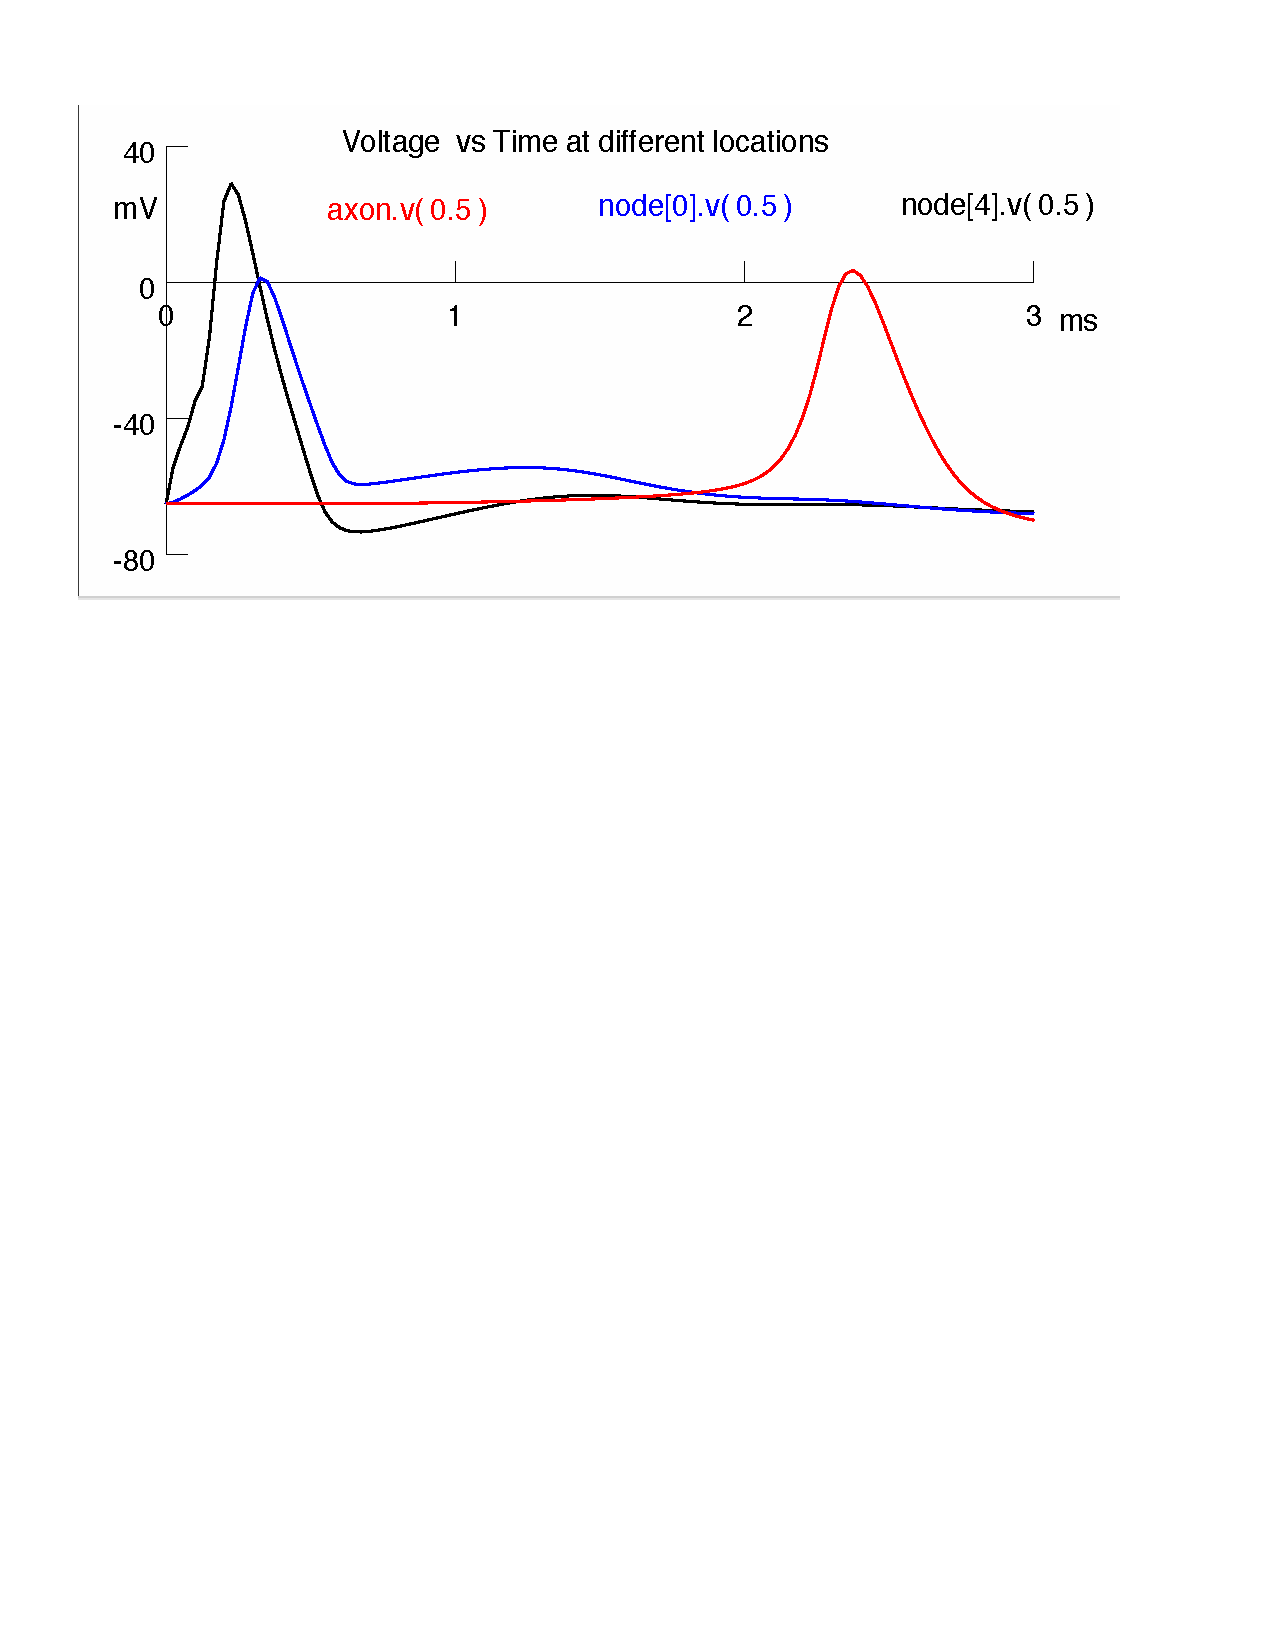
\includegraphics[width=0.9\textwidth]{Results/4a-03567}
\caption{\label{fig:P4a1} Partial Demyelination of the axon at a K+ Channel Density of $0.03567 \rfrac{S}{cm^{2}}$ is the maximum value at which an AP can propagate across the entire axon.}
\end{figure}


\slntParagraph{ As K+ Channel Density is reduced, the propagating wave loses less and less energy at the interface between the myelinated and bare portions of the axon. At a K+ Channel Density of $0.03567 \rfrac{S}{cm^{2}}$, the AP transitions to being able to propagate along the bare portion.}

\slntParagraph{ Decreasing K+ Channel Density even further (up to $0.001 \rfrac{S}{cm^{2}}$) results in a much slower propagation speed but a thicker peak in bare axon. The amplitude of the AP seems about the same.}


%% P3.B
\subQuestion{Diameter}

\begin{figure}[H]
\centering
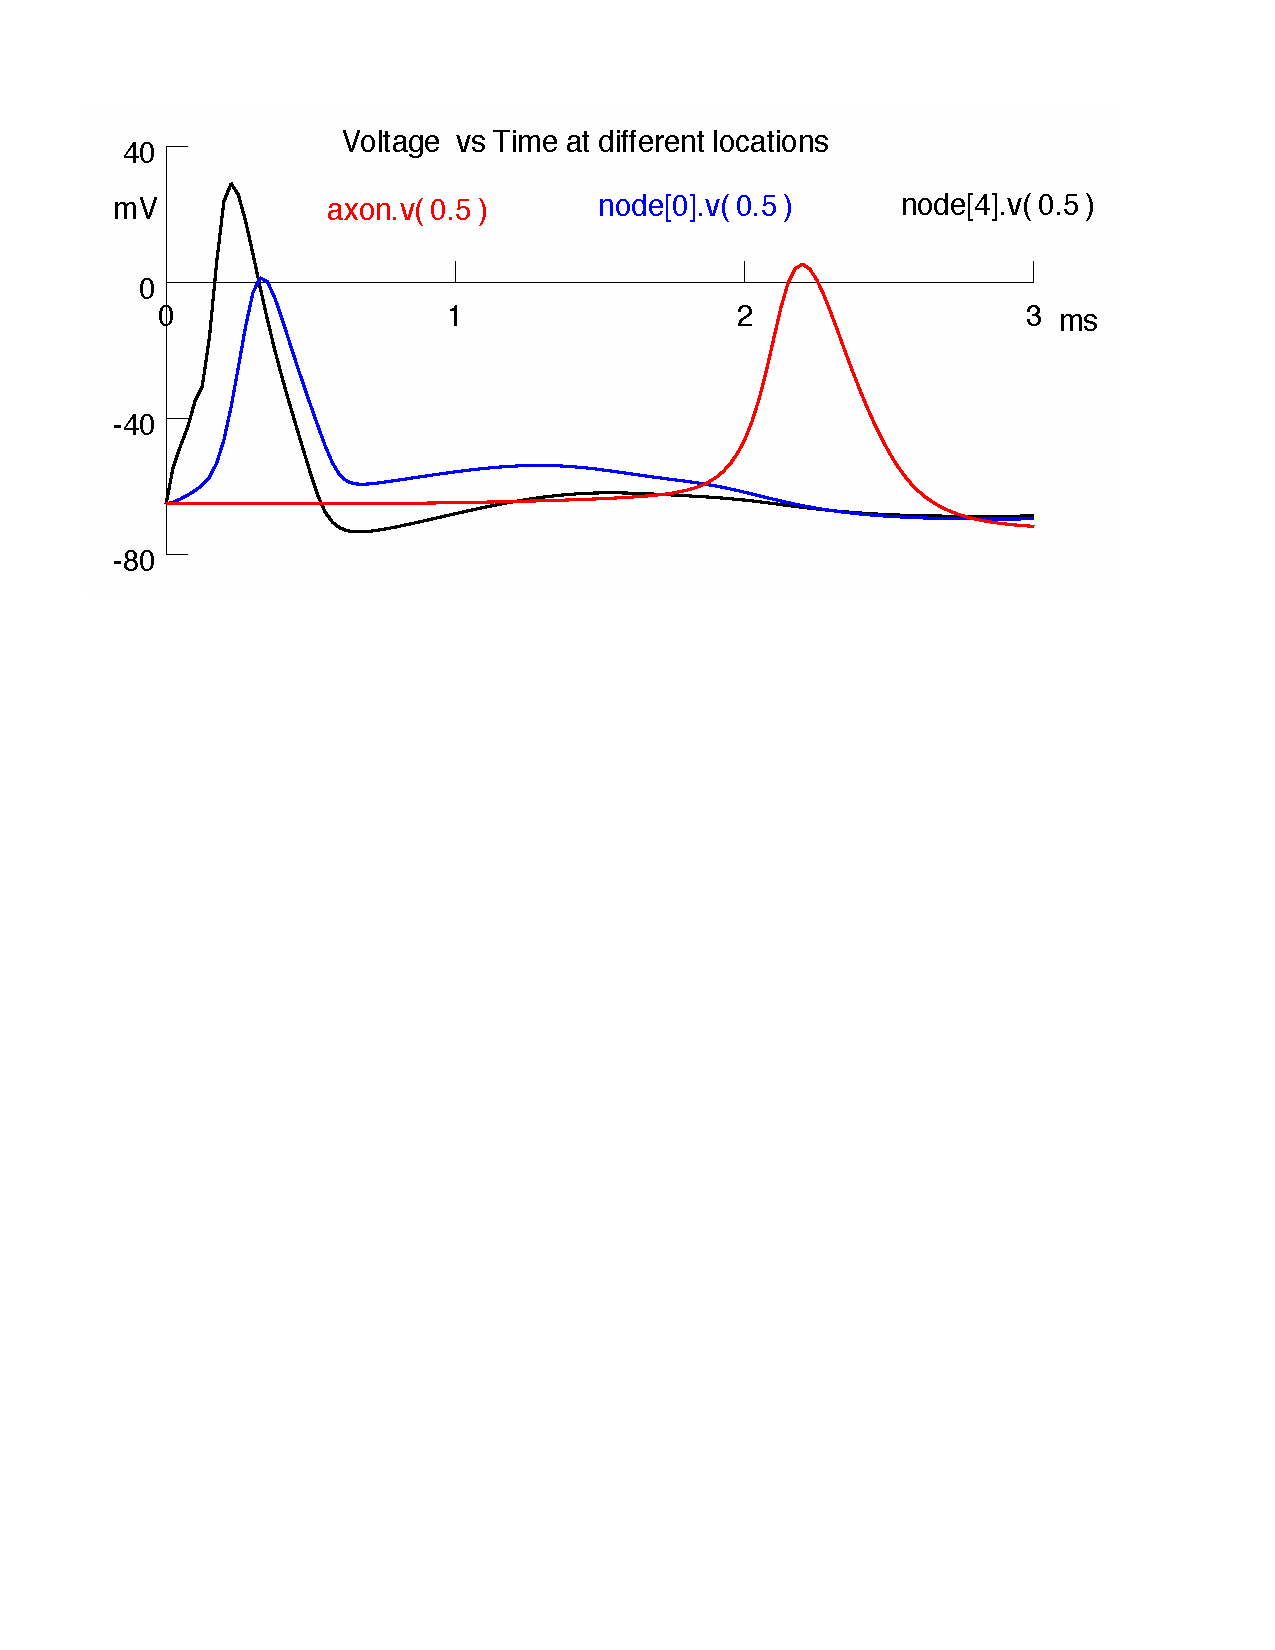
\includegraphics[width=0.9\textwidth]{Results/4b-997}
\caption{\label{fig:P4b1} Partial Demyelination of the axon at a diameter of $9.97 \mu m$ is the maximum value at which an AP can propagate across the entire axon.}
\end{figure}

\begin{figure}[H]
\centering
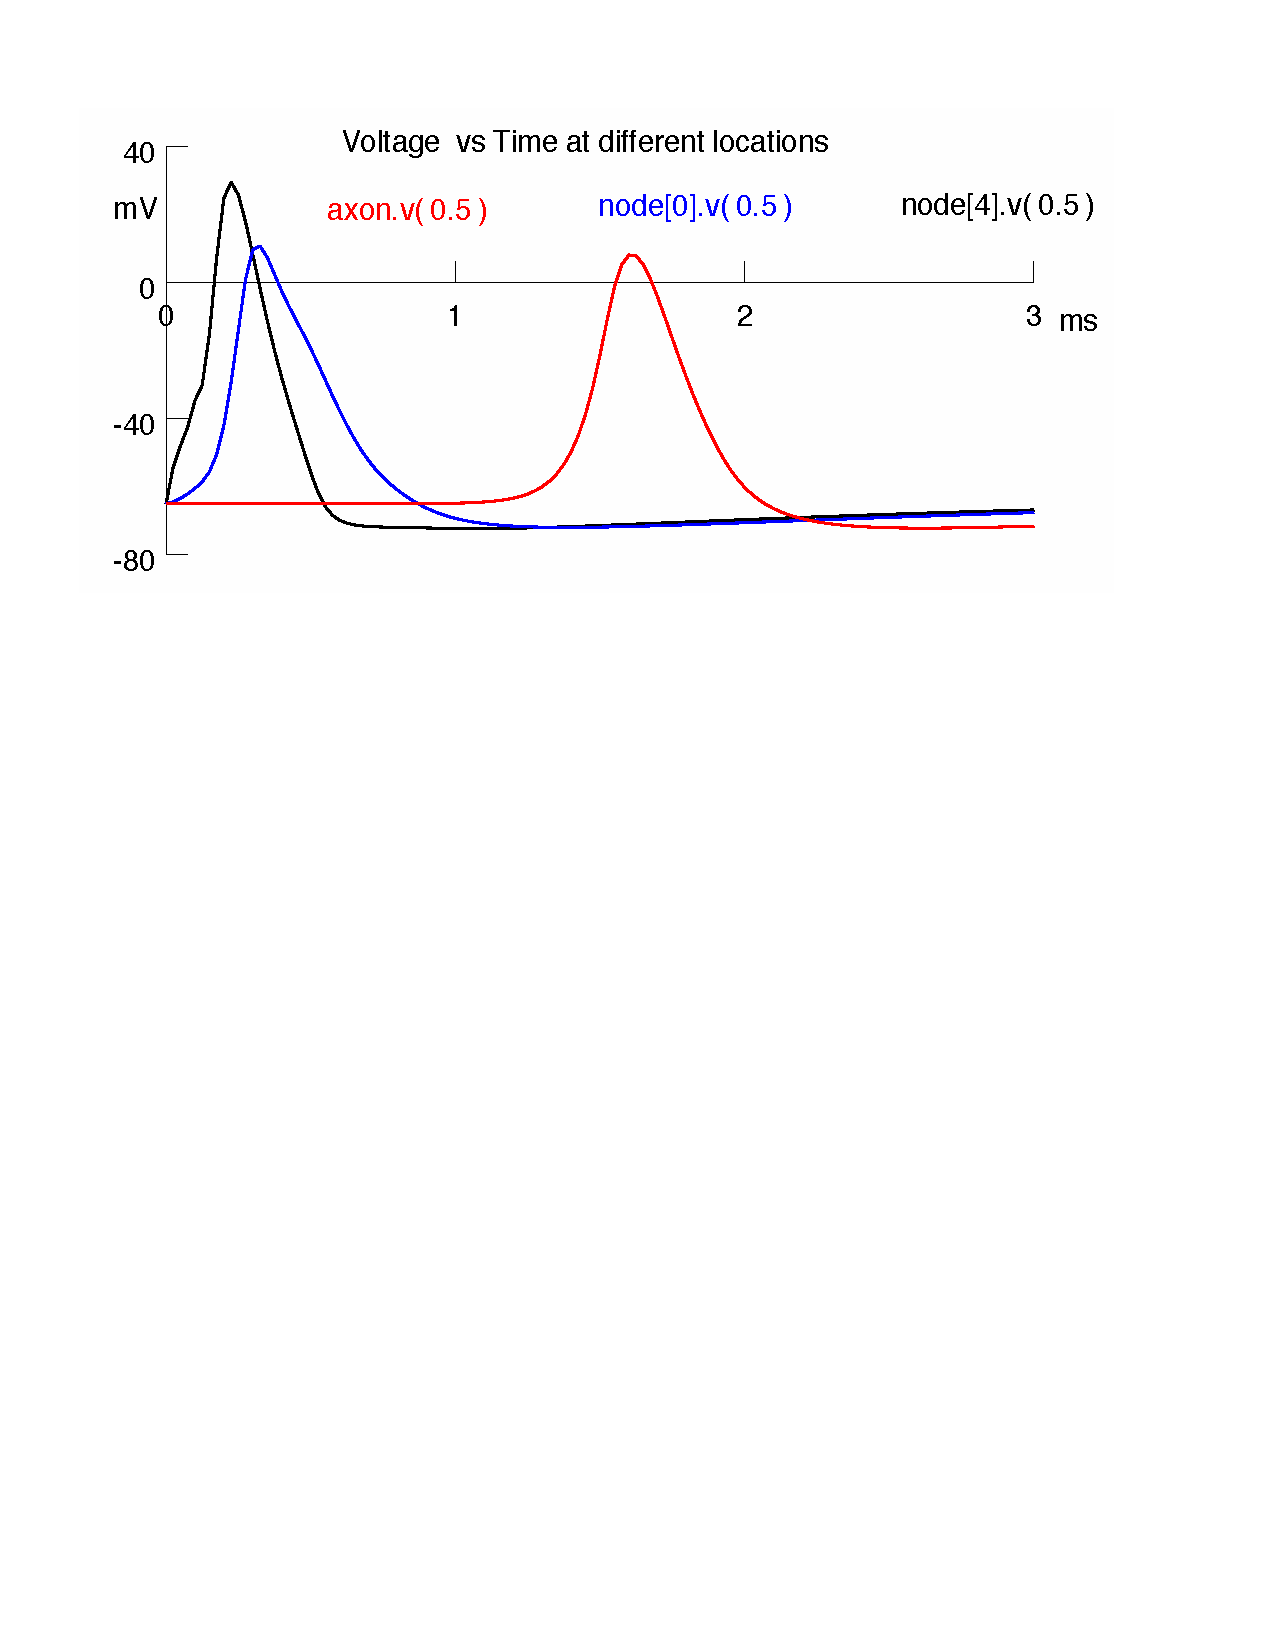
\includegraphics[width=0.9\textwidth]{Results/4b-5}
\caption{\label{fig:P4b2} Partial Demyelination of the axon at a diameter of $5.00 \mu m$ demonstrates the effect of further reduction of diameter on AP propagation dynamics.}
\end{figure}

\slntParagraph{As Diameter is reduced, it's found that the AP can begin to cross the interface around $9.97 \mu m$. Decreasing the diameter further results in a decrease in the maximum attained amplitude of the wave in the bare axon, and a decrease in the width of the peak (and an increase in its sharpness).}


%% P3.C
\subQuestion{Length of internode Myelin[0]}

\begin{figure}[H]
\centering
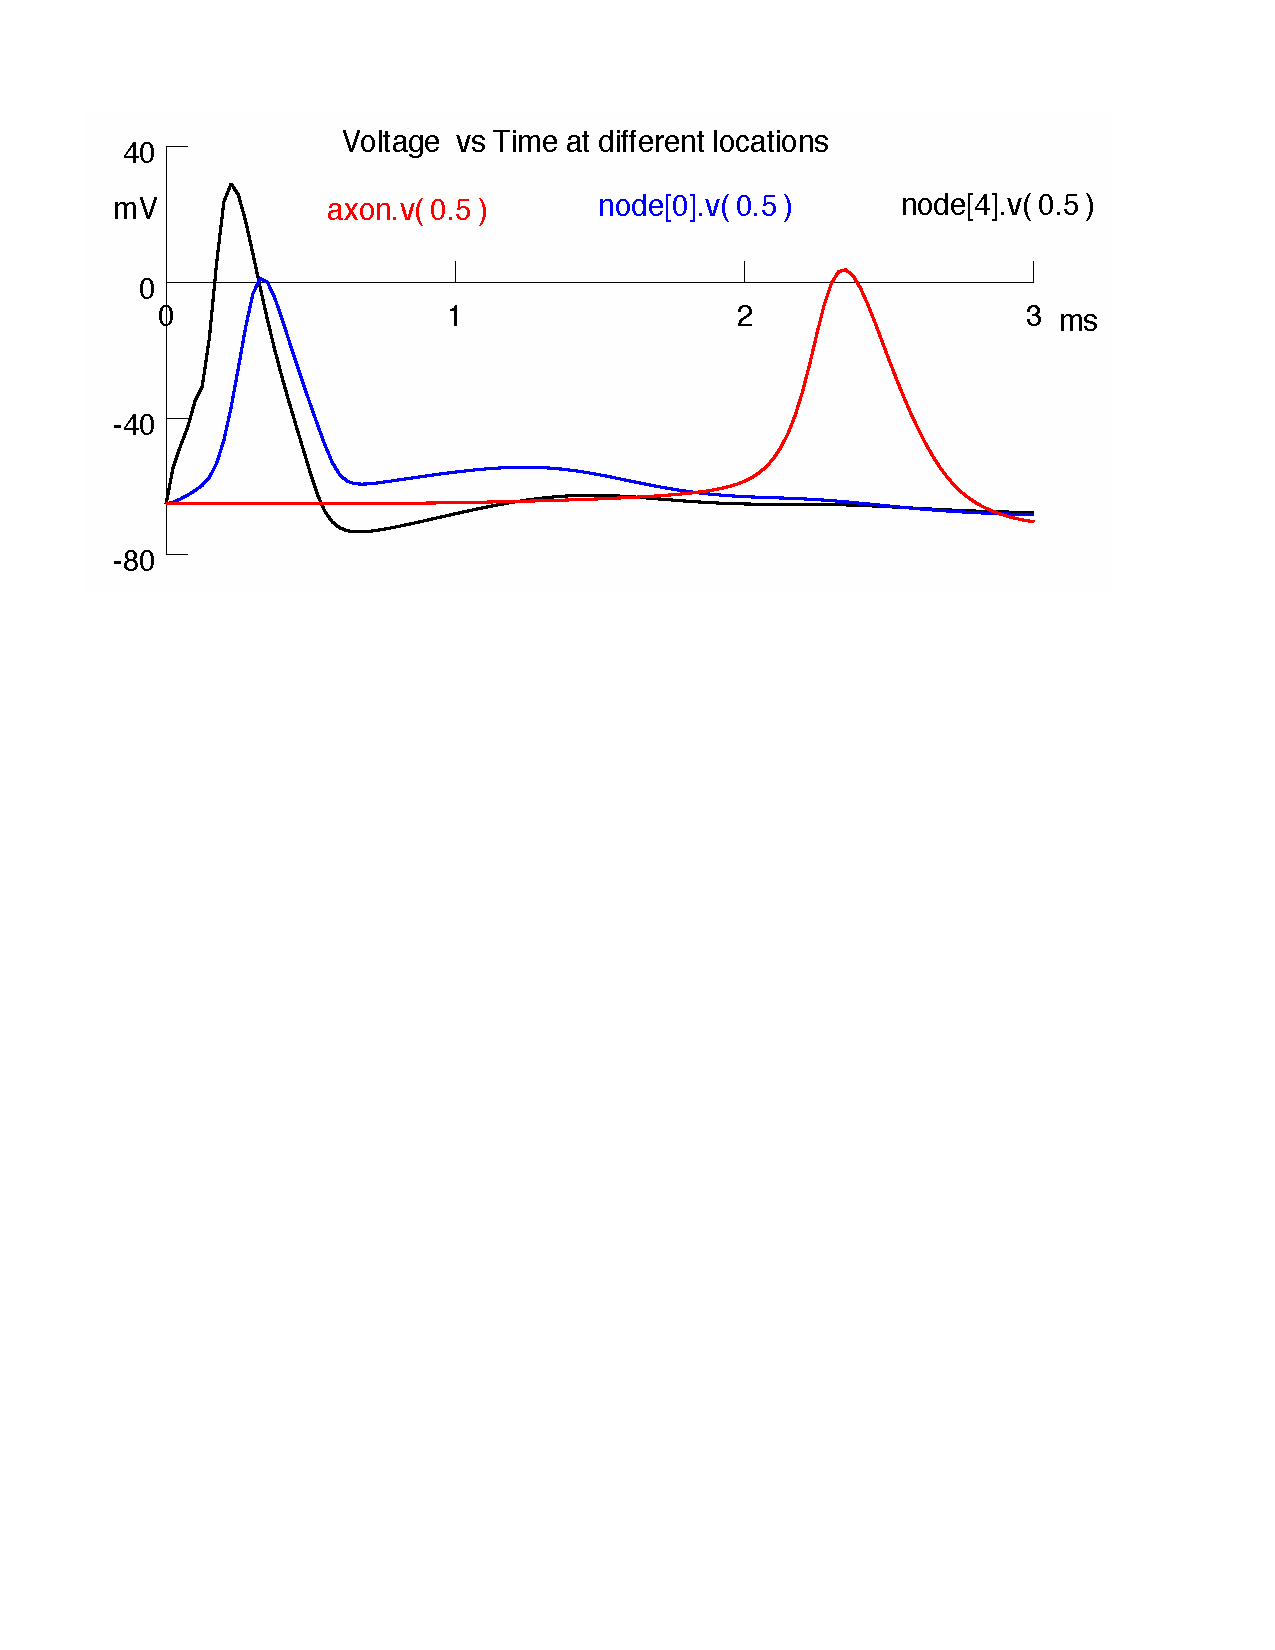
\includegraphics[width=0.9\textwidth]{Results/4c-993}
\caption{\label{fig:P4c1} Partial Demyelination of the axon with a length of internode Myelin[0] of $993 \mu m$ is the maximum value at which an AP can propagate across the entire axon.}
\end{figure}

\begin{figure}[H]
\centering
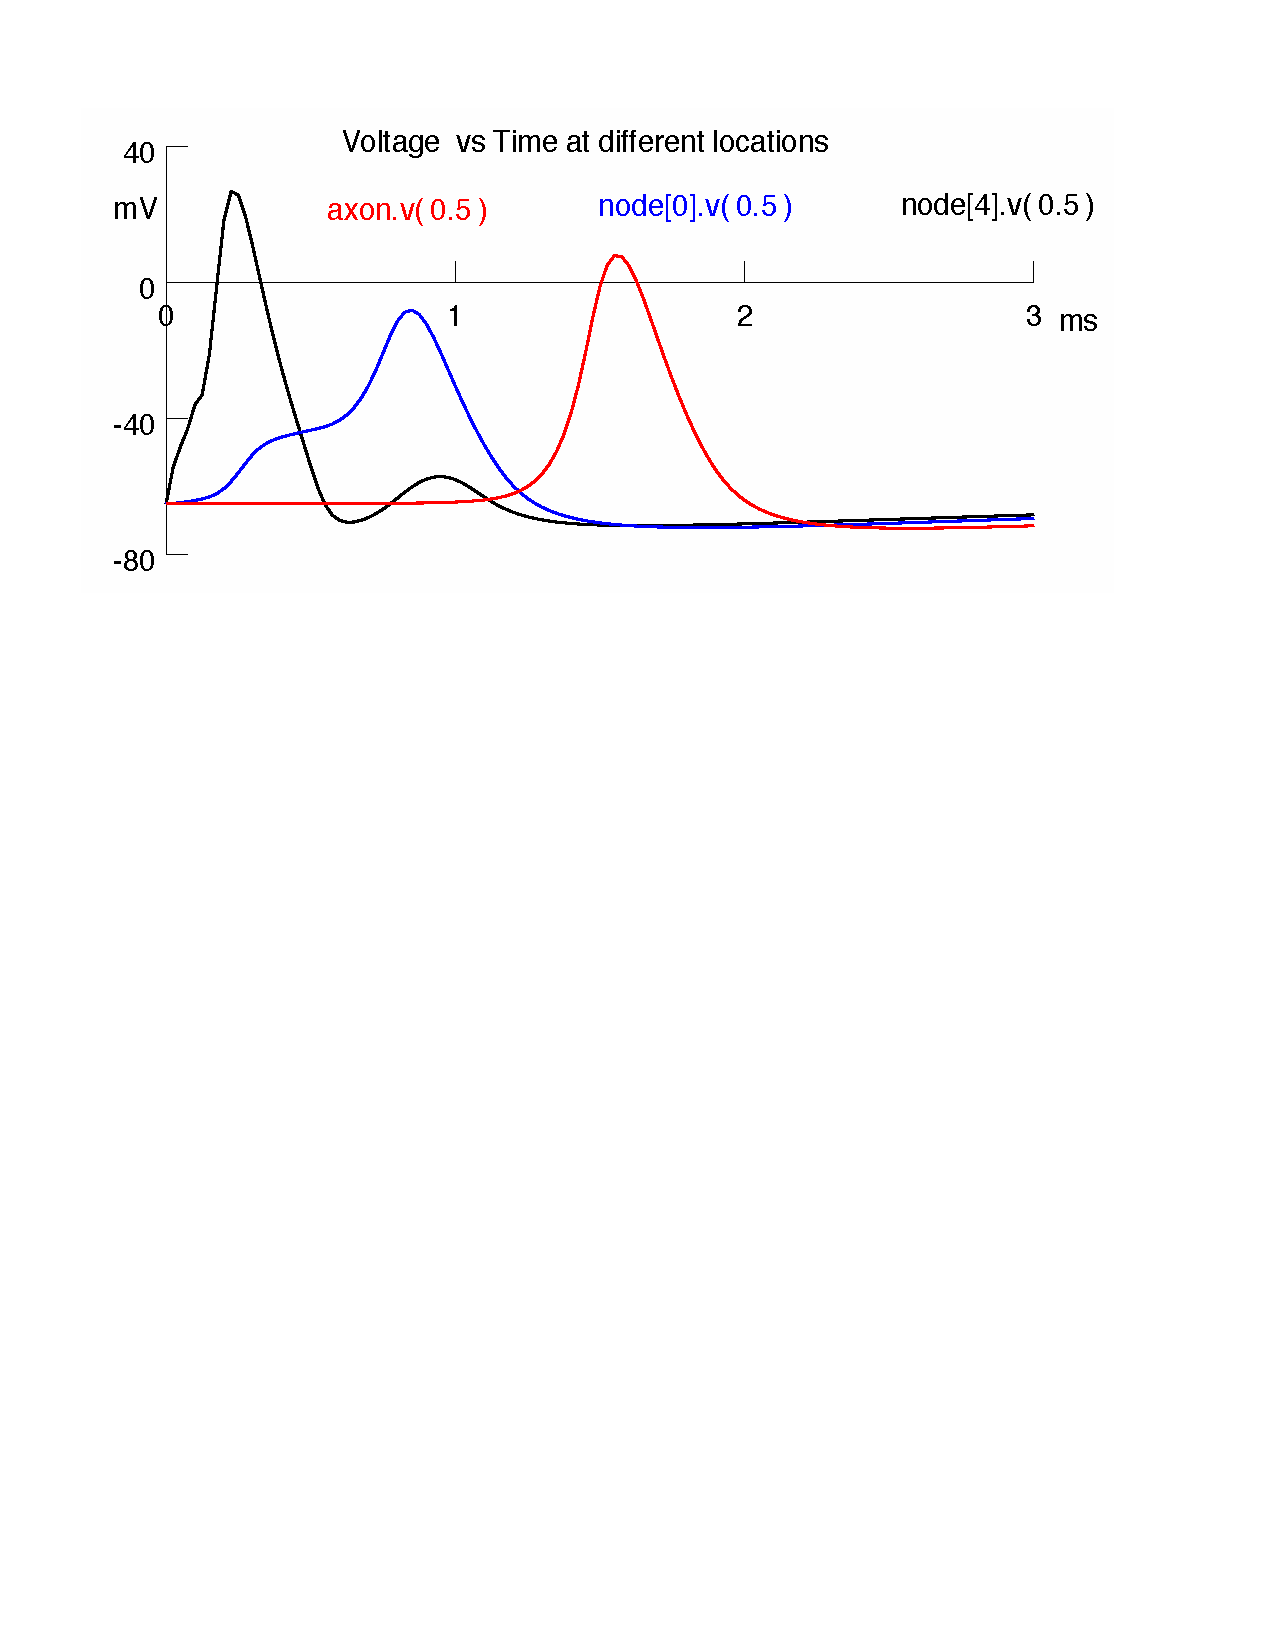
\includegraphics[width=0.9\textwidth]{Results/4c-1}
\caption{\label{fig:P4c2} Partial Demyelination of the axon with a short length of internode Myelin[0] of $1.0 \mu m$ demonstrates the effect of further reduction of internode Myelin[0] length on AP propagation dynamics. A low magnitude incoming wave is transmitted across the interface with a moderate delay, creating a relatively high magnitude and narrow propagating wave.}
\end{figure}


\begin{figure}[H]
\centering
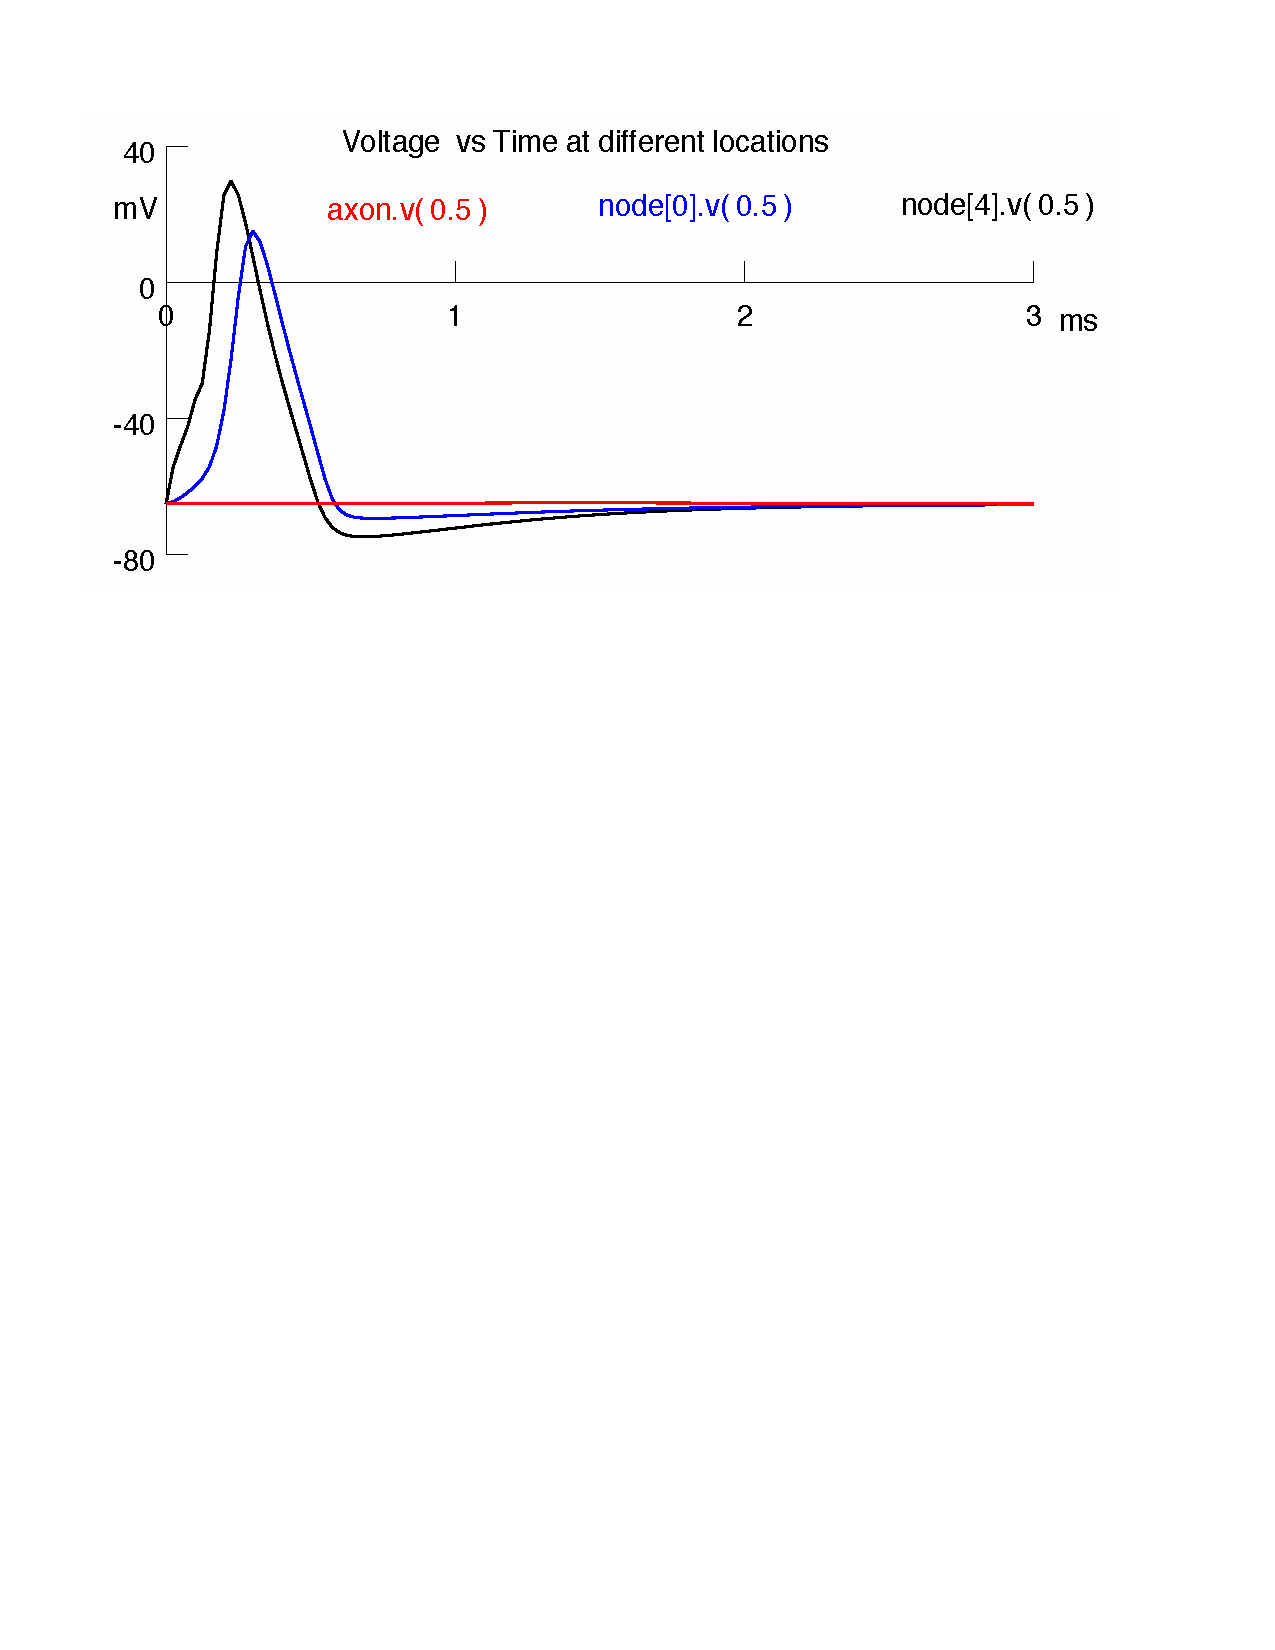
\includegraphics[width=0.9\textwidth]{Results/4c-2000}
\caption{\label{fig:P4c3} Partial Demyelination of the axon with a very long length of internode Myelin[0] of $2000 \mu m$ better demonstrates the effect that modulation of internode Myelin[0] length has on AP propagation dynamics. The bare end of the axon appears "heavy" to the propagating wave for large values of Myelin[0] length, and the AP is not successfully transmitted across the interface.}
\end{figure}



\slntParagraph{As the Length of internode Myelin[0] is reduced for its default value of $1000 \mu m$, it's found that the AP can begin to cross the interface around $993 \mu m$. To better demonstrate the effect the length of internode Myelin[0] has on AP dynamics, both high (see Figure \ref{fig:P4c3}) and low (see Figure \ref{fig:P4c2}) values were compared. The higher the length of internode Myelin[0], the less "heavy" the bare end of the axon appears to the propagating wave, and the longer it takes for the curve to completely "relax" back to baseline values despite the very low amplitude of change.}


%% P3.D
\subQuestion{Thickness of myelin sheath in Myelin[0]} 

\begin{figure}[H]
\centering
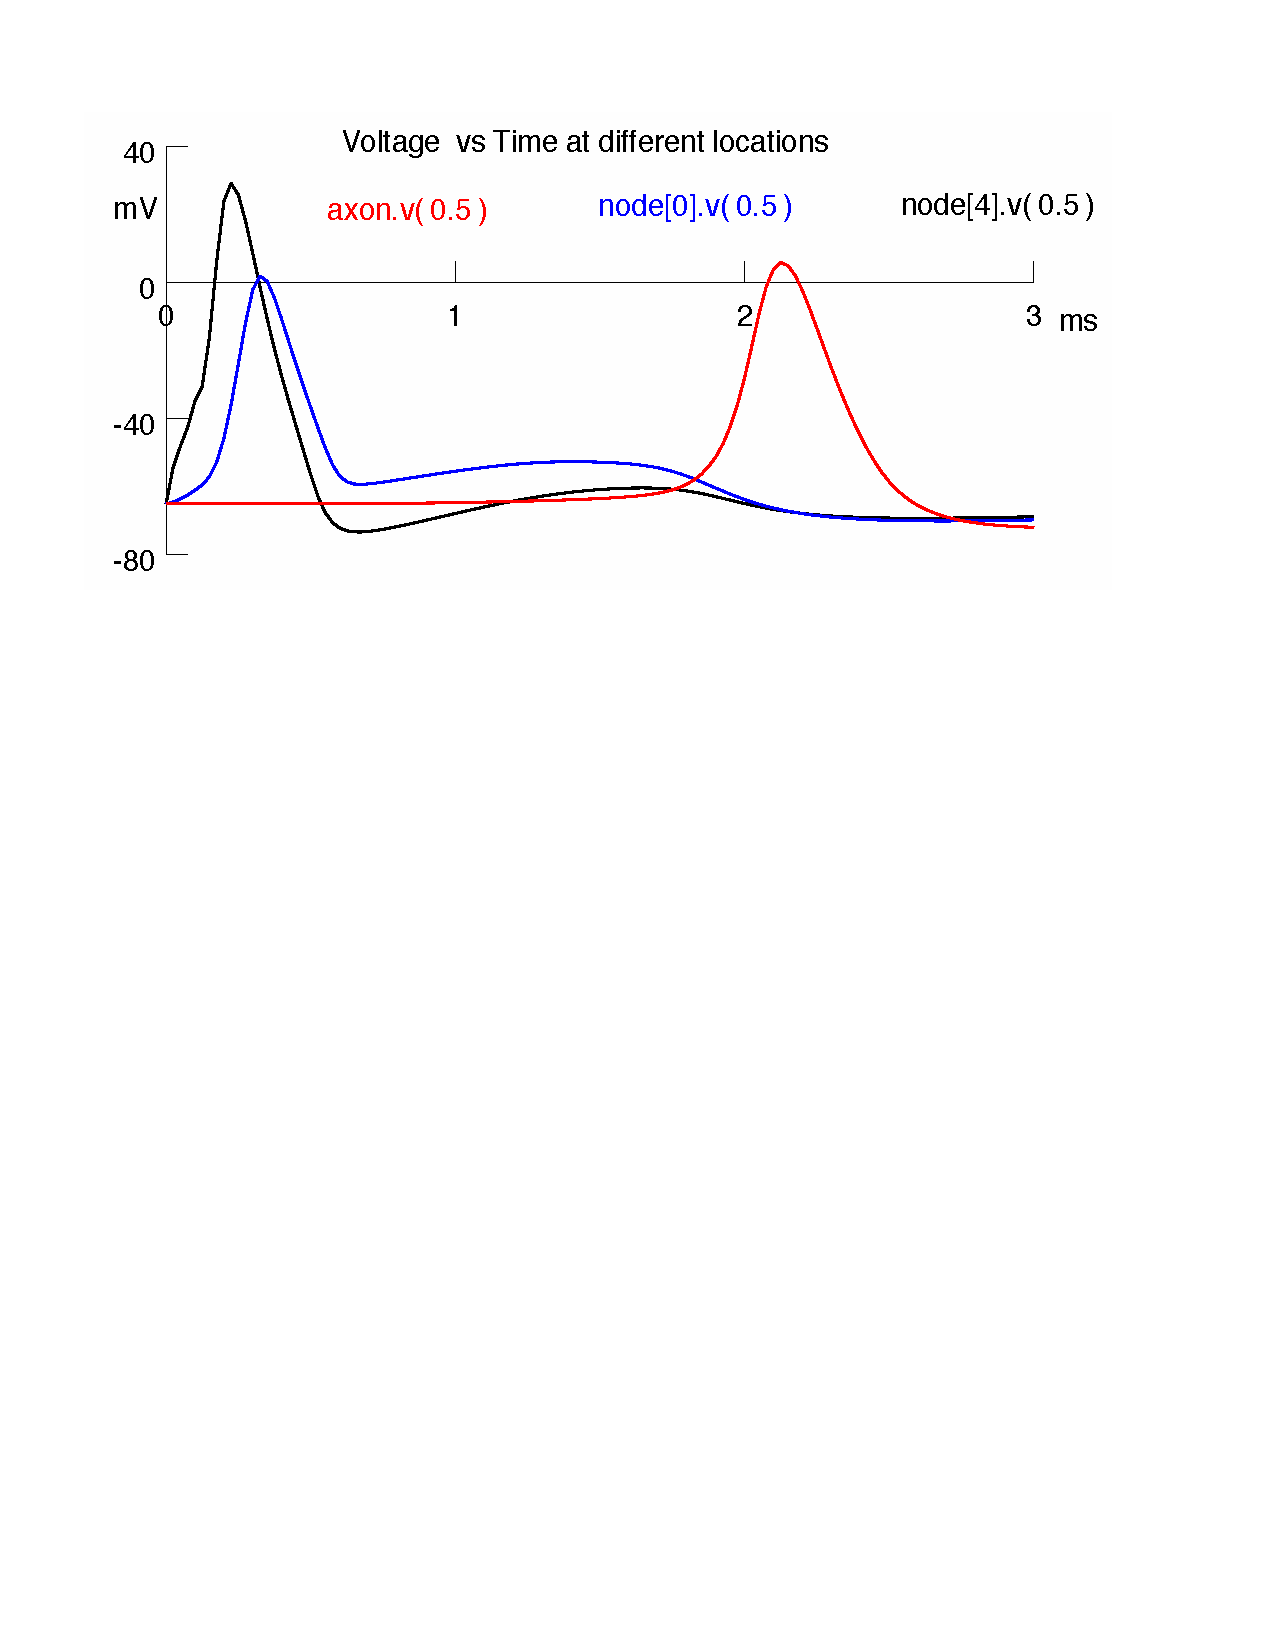
\includegraphics[width=0.9\textwidth]{Results/4d-002}
\caption{\label{fig:P4d1} Partial Demyelination of the axon with a Myelin[0] capacitance of $0.002 \rfrac{\mu F}{cm^{2}}$ is the maximum value at which an AP can propagate across the entire axon.}
\end{figure}

\begin{figure}[H]
\centering
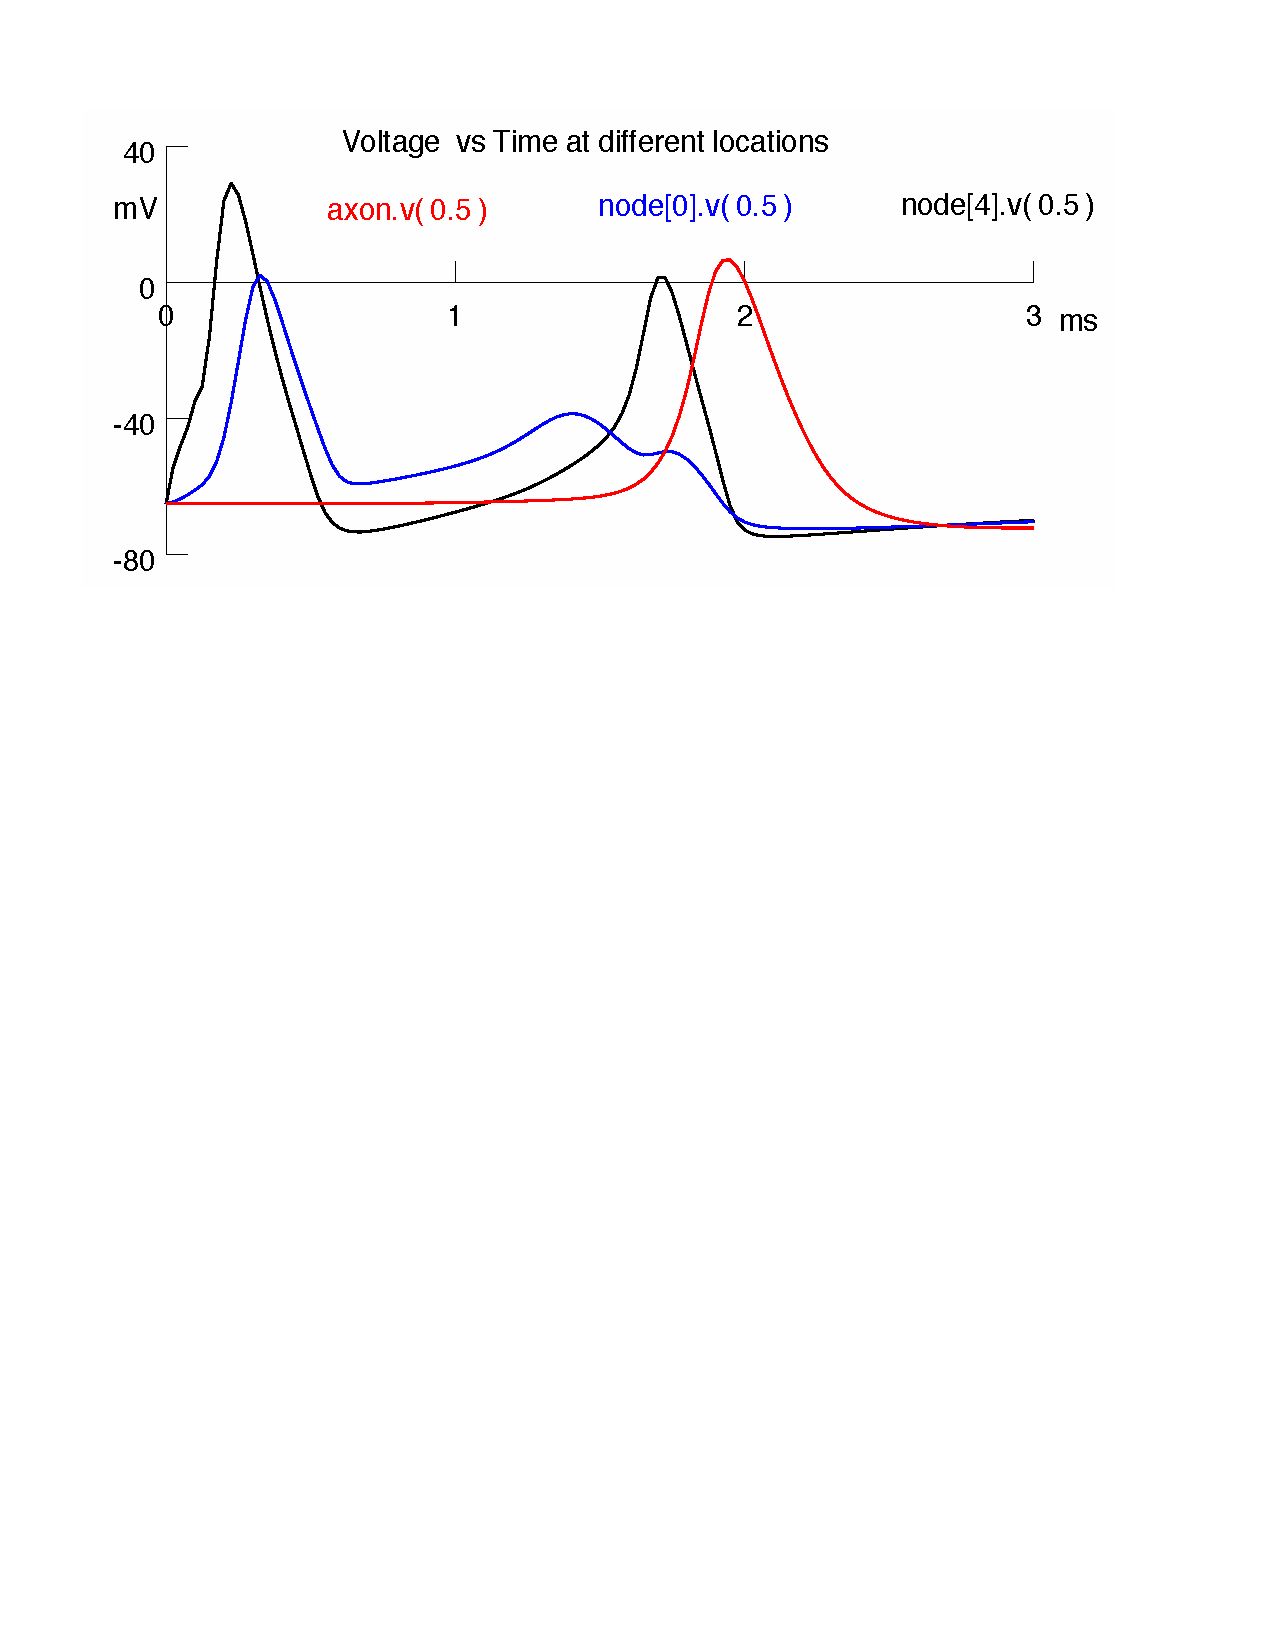
\includegraphics[width=0.9\textwidth]{Results/4d-0001}
\caption{\label{fig:P4d2} Partial Demyelination of the axon with a Myelin[0] capacitance (as a stand-in for sheath thickness) of $0.0001 \rfrac{\mu F}{cm^{2}}$ demonstrates the effect of further reduction of Myelin[0] capacitance on AP propagation dynamics. A substantial "reflection" is observed at the interface, with some of the energy propagating backwards back towards the stimulation point.}
\end{figure}

\slntParagraph{Finally, the thickness of the myelin sheath in Myelin[0] was modulated by changing the capacitance for that segment. As the capacitance was reduced from its default value of $0.005 \rfrac{\mu F}{cm^{2}}$, it was found that the AP can begin to cross the interface around $0.002 \rfrac{\mu F}{cm^{2}}$ as shown in Figure $\ref{fig:P4d1}$. It was observed that further decreasing the capacitance caused a substantial "bounce back" of the propagating wave (reflection). It appeared as if the amount of energy transmitted through the interface was limited to around the value that caused the AP, while any excess was reflected backwards. This is demonstrated in Figure $\ref{fig:P4d2}$, where a substantial reflection occurs for capacitance values of $0.0001 \rfrac{\mu F}{cm^{2}}$. }



\end{document}
